\documentclass[conference]{IEEEtran}
\IEEEoverridecommandlockouts
\usepackage{blindtext}
\usepackage{gensymb}
\usepackage{graphicx}
\graphicspath{ {./images/}  }

\begin{document}

\title{ECSE 331\\
    Laboratory No. 2\\
    Simulation of semiconductor diode in PSPICE\\
    \Large \today\\
}

\author
{
    \IEEEauthorblockN{Seyed Yazdan Zinati}
    \IEEEauthorblockA{260928077 \\
    \textit{seyed.zinati@mail.mcgill.ca}}

    \and

    \IEEEauthorblockN{James Wu}
    \IEEEauthorblockA{260929944 \\
    \textit{james.wu4@mail.mcgill.ca}}
}
\maketitle
\clearpage

\begin{abstract}
    A diode is a two-terminal semiconductor device that conducts current primarily in one direction. Despite being simple two-pin devices, their applications such as voltage rectification, signal mixing, signals isolation, and lighting make them vital in electronics. Diodes have become an essential part of all electronics. As the complexity of electronic devices increases, designing circuits by hand becomes an impossible task due to being very time-consuming and prone to human errors. Consequently, engineers design intricate circuits using circuit simulation software such as SPICE. In this laboratory, we design and simulate diode circuits to analyze their characteristics and some of their applications in electronic circuits. This includes analyzing diode specifications such as the cut-off voltage, Zener breakdown, conduction in forward bias, and the effect of temperature on diode characteristics. We then build and simulate circuits using diodes, namely a full-wave bridge rectifier and a clipper circuit.
\end{abstract}

\section{Introduction}
A diode is a two-terminal semiconductor device that conducts current primarily in one direction. It is essentially a one-way current switch. It has a low resistance in one direction and high resistance in the other. The diode allows current to flow in forward-biased whereas, in reverse-bias, the diode blocks the current flow.

In this laboratory, we conduct experiments on five circuits to get familiarized with the use of simulation software in designing and analyzing circuits consisting of diodes. We first study the cut-off voltage of a silicon diode and investigate the effect that temperature has on it. We then build and analyze three different circuits that show the application of diodes, particularly two different full-wave bridge rectifiers and a clipper circuit. Finally, we study some of the characteristics of a Zener diode

\subsection*{Task 1}
This experiment required using PSPICE to build the circuit shown in Figure 1 and to find the cut-off voltage of the diode by plotting the variation of current through the diode with respect to the voltage across it.

\begin{figure}[h]
    \caption{Task 1 circuit}
    \centering
    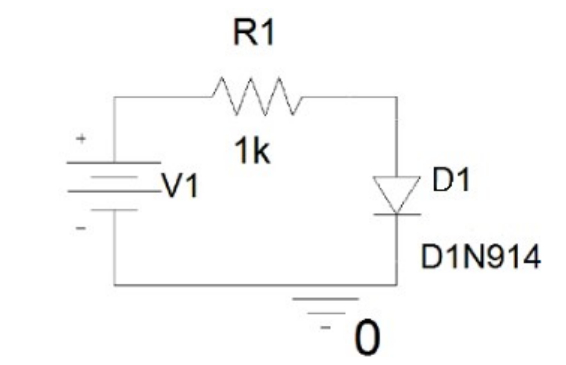
\includegraphics[scale=0.4]{fig1}
\end{figure}

\subsection*{Task 2}
In this experiment, we study the effect of temperate on diode characteristics by finding the I-V plot at 50 \degree C, 100 \degree C, and 150 \degree C.

\subsection*{Task 3}
In this experiment, we construct a full-wave bridge rectifier circuit shown in Figure 2. We then have to plot the voltage V1 and the output voltage across R1 versus time.

\begin{figure}[h]
    \caption{Full Wave bridge rectifier}
    \centering
    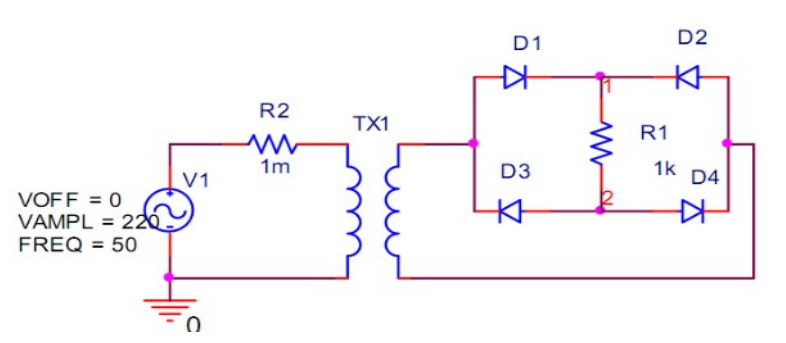
\includegraphics[scale=0.3]{fig2}
\end{figure}
\subsection*{Task 4}
In this experiment, we add a capacitor in parallel to the R1 resistor in the circuit shown in Figure 2. Again, we plot the output voltage across R1 across time by experimenting with three different capacitor values.

\subsection*{Task 5}
In this experiment, we build the clipper circuit shown in Figure 3. We choose the values of V1 and V2 such that the output voltage V0 is as follows:\\

\noindent V0 = Vin for -5V\textless Vin\textless 9V\\
V0 = 9V for Vin \textgreater 9V\\
V0 = -5V for Vin\textless -5V
\\

This simulation is then followed by a theoretical discussion.

\begin{figure}[h]
    \caption{Clipper circuit}
    \centering
    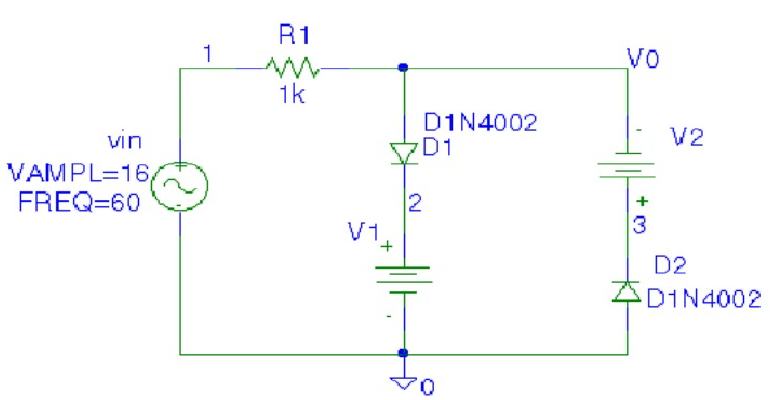
\includegraphics[scale=0.33]{fig3}
\end{figure}
\subsection*{Task 6}
\begin{figure}[h]
    \caption{Zener diode circuit}
    \centering
    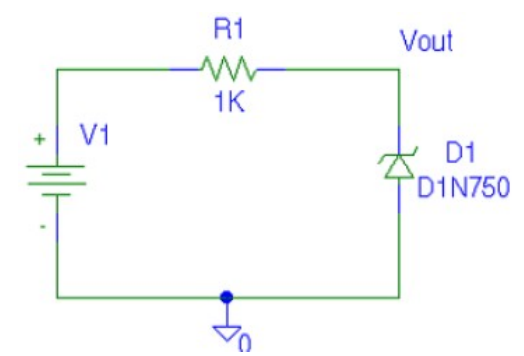
\includegraphics[scale=0.3]{fig4}
\end{figure}
In this experiment, we construct the circuit shown in Figure 4. We plot the variation of current across the Zener diode with respect to the variation of voltage to find the voltage at which the Zener breakdown occurs and the voltage at which the diode starts to conduct in the forward bias region.

\section{Solutions}
\blindtext
\end{document}
